\documentclass[12pt]{article}

\usepackage[usenames]{color}
\definecolor{gray}{rgb}{.8,.8,.8}


\usepackage{graphicx}
\DeclareGraphicsExtensions{.eps, .ps, .pdf}

\usepackage{calc}


\usepackage{hyperref}


\usepackage{listings}
\lstset{ %
language=Octave,                % the language of the code
basicstyle=\footnotesize,       % the size of the fonts that are used for the code
numbers=none,                   % where to put the line-numbers
numberstyle=\footnotesize,      % the size of the fonts that are used for the line-numbers
stepnumber=2,                   % the step between two line-numbers. If it's 1, each line 
                                % will be numbered
numbersep=5pt,                  % how far the line-numbers are from the code
backgroundcolor=\color{gray},  % choose the background color. You must add \usepackage{color}
showspaces=false,               % show spaces adding particular underscores
showstringspaces=false,         % underline spaces within strings
showtabs=false,                 % show tabs within strings adding particular underscores
frame=single,                   % adds a frame around the code
tabsize=2,                      % sets default tabsize to 2 spaces
captionpos=b,                   % sets the caption-position to bottom
breaklines=true,                % sets automatic line breaking
breakatwhitespace=false,        % sets if automatic breaks should only happen at whitespace
title=\lstname,                 % show the filename of files included with \lstinputlisting;
                                % also try caption instead of title
escapeinside={\%*}{*)},         % if you want to add a comment within your code
morekeywords={*,...}            % if you want to add more keywords to the set
}



\textwidth=16.25cm
\textheight=22.7cm
\oddsidemargin=0.1cm
\topmargin=0.35in
\headsep=0.5cm


\newcommand{\as}[2]{\mbox{#1\farcs #2}}
\newcommand{\am}[2]{$#1^{'}\,\hspace{-1.7mm}.\hspace{.1mm}#2$}
\newcommand{\HI}{\mbox{H\,{\sc i}}}
\newcommand{\kms}{\mbox{\rm km\,s$^{-1}$}}
\newcommand{\SK}{$S^{3}$}
\def\lsim{~\rlap{$<$}{\lower 1.0ex\hbox{$\sim$}}}
\def\gsim{~\rlap{$>$}{\lower 1.0ex\hbox{$\sim$}}}

\title{Manual for the HART Software Package}
\author{Mark Benjamin \& Leonid Benkevich}

\begin{document}
\maketitle
\bigskip

\begin{figure}[htb]
\begin{center}
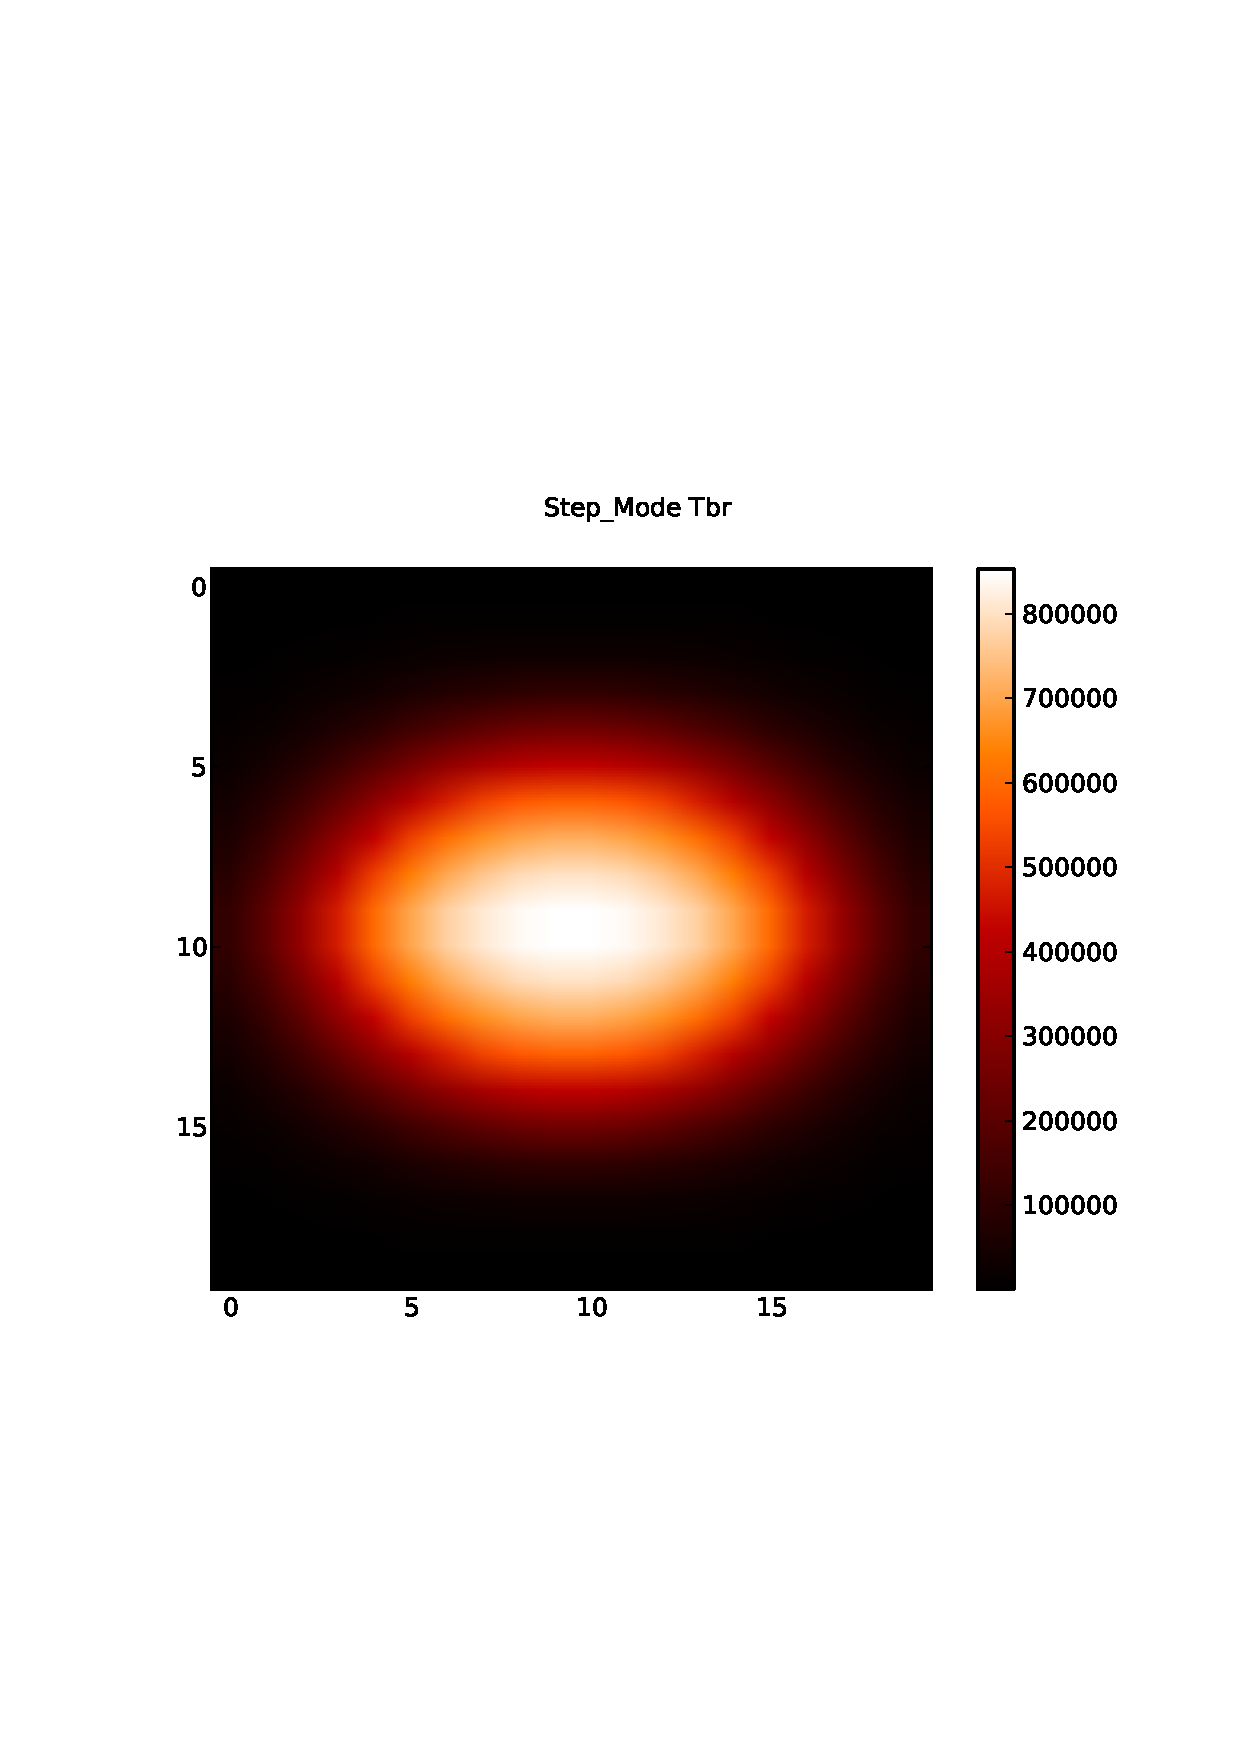
\includegraphics[scale=.75]{tbr}
\end{center}
\end{figure}

\centerline{\large\bf MASSACHUSETTS INSTITUTE OF TECHNOLOGY}
\centerline{\large\bf HAYSTACK OBSERVATORY}
\smallskip
\centerline{\normalsize Westford, Massachusetts 01886}
\newpage

\tableofcontents

\newpage

\section{Introduction}
The HART software suite focuses on providing a comprehensive
package to perform raytracing in the Solar Corona. This
suite comes at a pertinent time considering the current construction of the
Murchison Widefield Array (MWA) in Australia. As the MWA comes online,
there will be new solar data that can be compared with our current
models. This software package facilitates this comparision by
including a GUI, speed improvements via multi-threading and CUDA, and
an improved raytracing algorithm.

Written in C and Python, HART combines computational speed, with ease
of use. Using the matplotlib package for python, simulations can be
run and instantly graphed. By using the pyfits package fits files
can be created for a range of frequency simulations. It is with these
advantages that HART attempts to probe the depths of the Solar Corona.



\section{The Algorithm}

\section{Using ipython}
Implementing the pylab package makes HART very compatible with ipython
(the interactive Python shell). Although HART comes with a GUI there
are sometimes advantages to running the program through ipython. We
will go through an example to show how one can use ipython to
dynamically interact with a raytracing simulation. 
\subsection{The First Simulation}


Running:
\begin{lstlisting}
ipython -pylab
\end{lstlisting}
will launch ipython while importing all of the pylab libraries which
are required for the raytracing simulation. Once launched run the
following commands.
\lstset{language=python}
\begin{lstlisting}
import raytrace as rt
rt.implane?
\end{lstlisting}
The implane class is the interface between the user and the
simulation. Running rt.implane? displays the classes, parameters, and
documentation. 


Now to actually create and run a simulation:
\begin{lstlisting}
implane = rt.implane()
implane.trace(1500)
imshow(implane.tbr)
colorbar()
\end{lstlisting}
While running you will see the status of the simulation progress until
all the rays have been fully traced. Calling imshow(implane.tbr) uses
matplotlib (part of the SciPy package) to display the data.

\begin{figure}[h]
\begin{center}
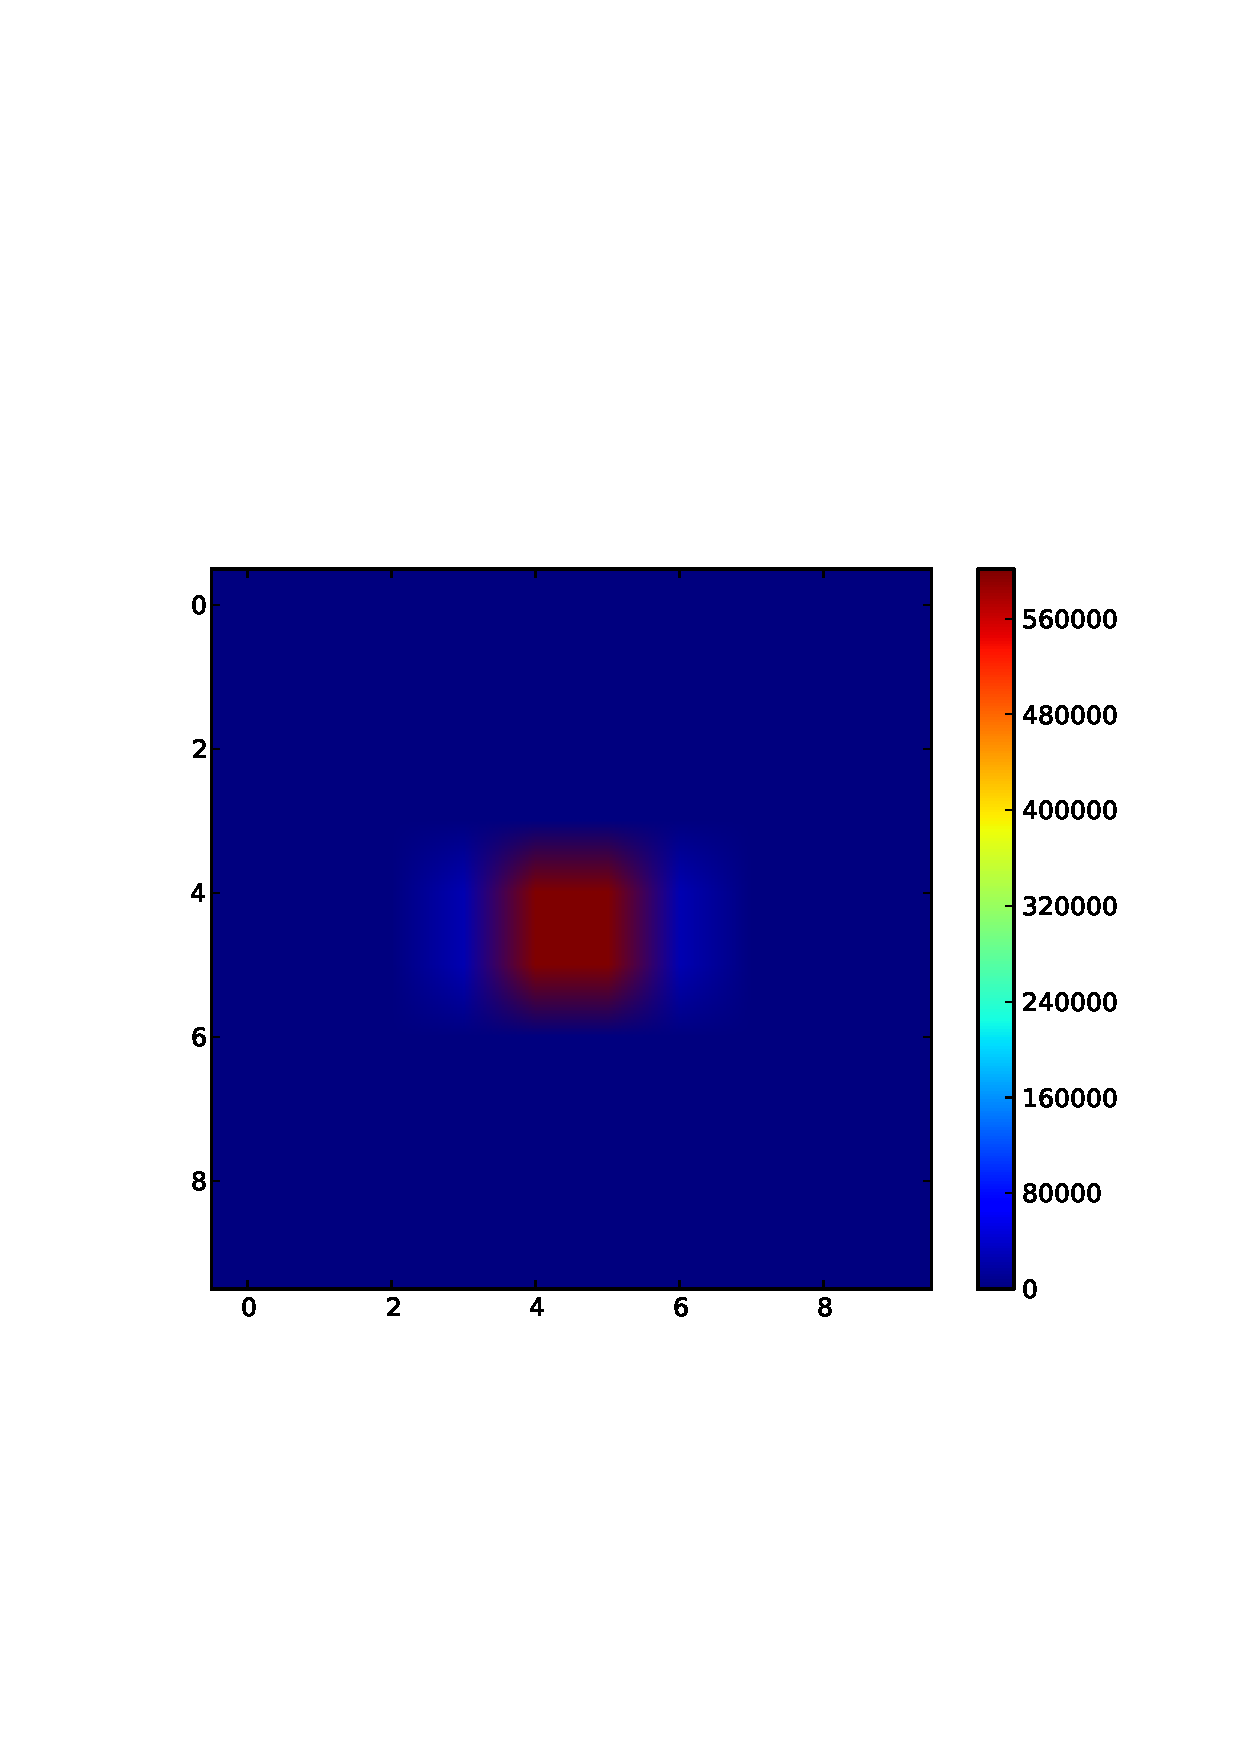
\includegraphics[scale=.75]{first_tbr}
\end{center}
\caption{Our first raytracing of the sun! However, this first image is
obviously not quite as accurate as we would like. In the next section
we will address the parameters that can make a better image.}
\end{figure}

\subsection{Adjusting the Raytracing Parameters}
\label{params}

Once again we'll begin by running
\begin{lstlisting}
import raytrace as rt
rt.implane?
\end{lstlisting}
Now let's consider the basic parameters that can be altered to customize the
raytracing.

\begin{itemize}
\item Grid=(width,height): Composed of a tupple of two
  dimmensions. This represents the grid over the sun from which the
  rays are launched from. In other words width by height is the
  resolution of the simulation to be preformed. Of course larger 
  resolutions take longer to complete.

\item Rect=($x_0,y_0,x_1,y_1$): This specifies the dimension of the
  rectangle from which the rays are launched from. The parameters are
  specified in terms of (optical) solar radii. So if rect is given as 
  (-1,-1,1,1) then the sun will consume the entire image plane. If 
  rect is instead (-5,-5,5,5) then the sun will only consume 1/5 of 
  the entire image plane.
 
\item Freq: This specifies the frequency in Hertz to run the
  simulation at.

\item Mode: This specifies how the simulation should be
  calculated. Three modes currently exist.
  \begin{itemize}
    \item 'Basic': This mode only calculates the trajectories of the
      rays, but not the brightness temperature or stokes parameters.
    \item 'Tbr': This mode calculates the brightness temperature of
      the rays.
    \item 'TbrIV': This mode calculates the stokes I and V of the
      rays.
  \end{itemize}

\item Units: This specifies whether the simulation should calculate
  values in terms of Kelvins or Janskys. 'K' for Kelvins, 'Jy' for Janskys.

\item Scattering: This specifies whether the rays will be scattered
  while being traced. True for scattering. False for no scattering.

\end{itemize}

\subsection{Performing a Customized Simulation}
Now we will run a simulation changing some of the parameters. Run the
following in the ipython window:
\begin{lstlisting}
import raytrace as rt
implane = rt.implane(grid=(100,100),rect=(-2,-2,2,2),freq=300e6)
implane.trace(1500)
imshow(implane.tbr,cmap=cm.gist_heat)
colorbar()
\end{lstlisting}

\begin{figure}[ht]
\begin{center}
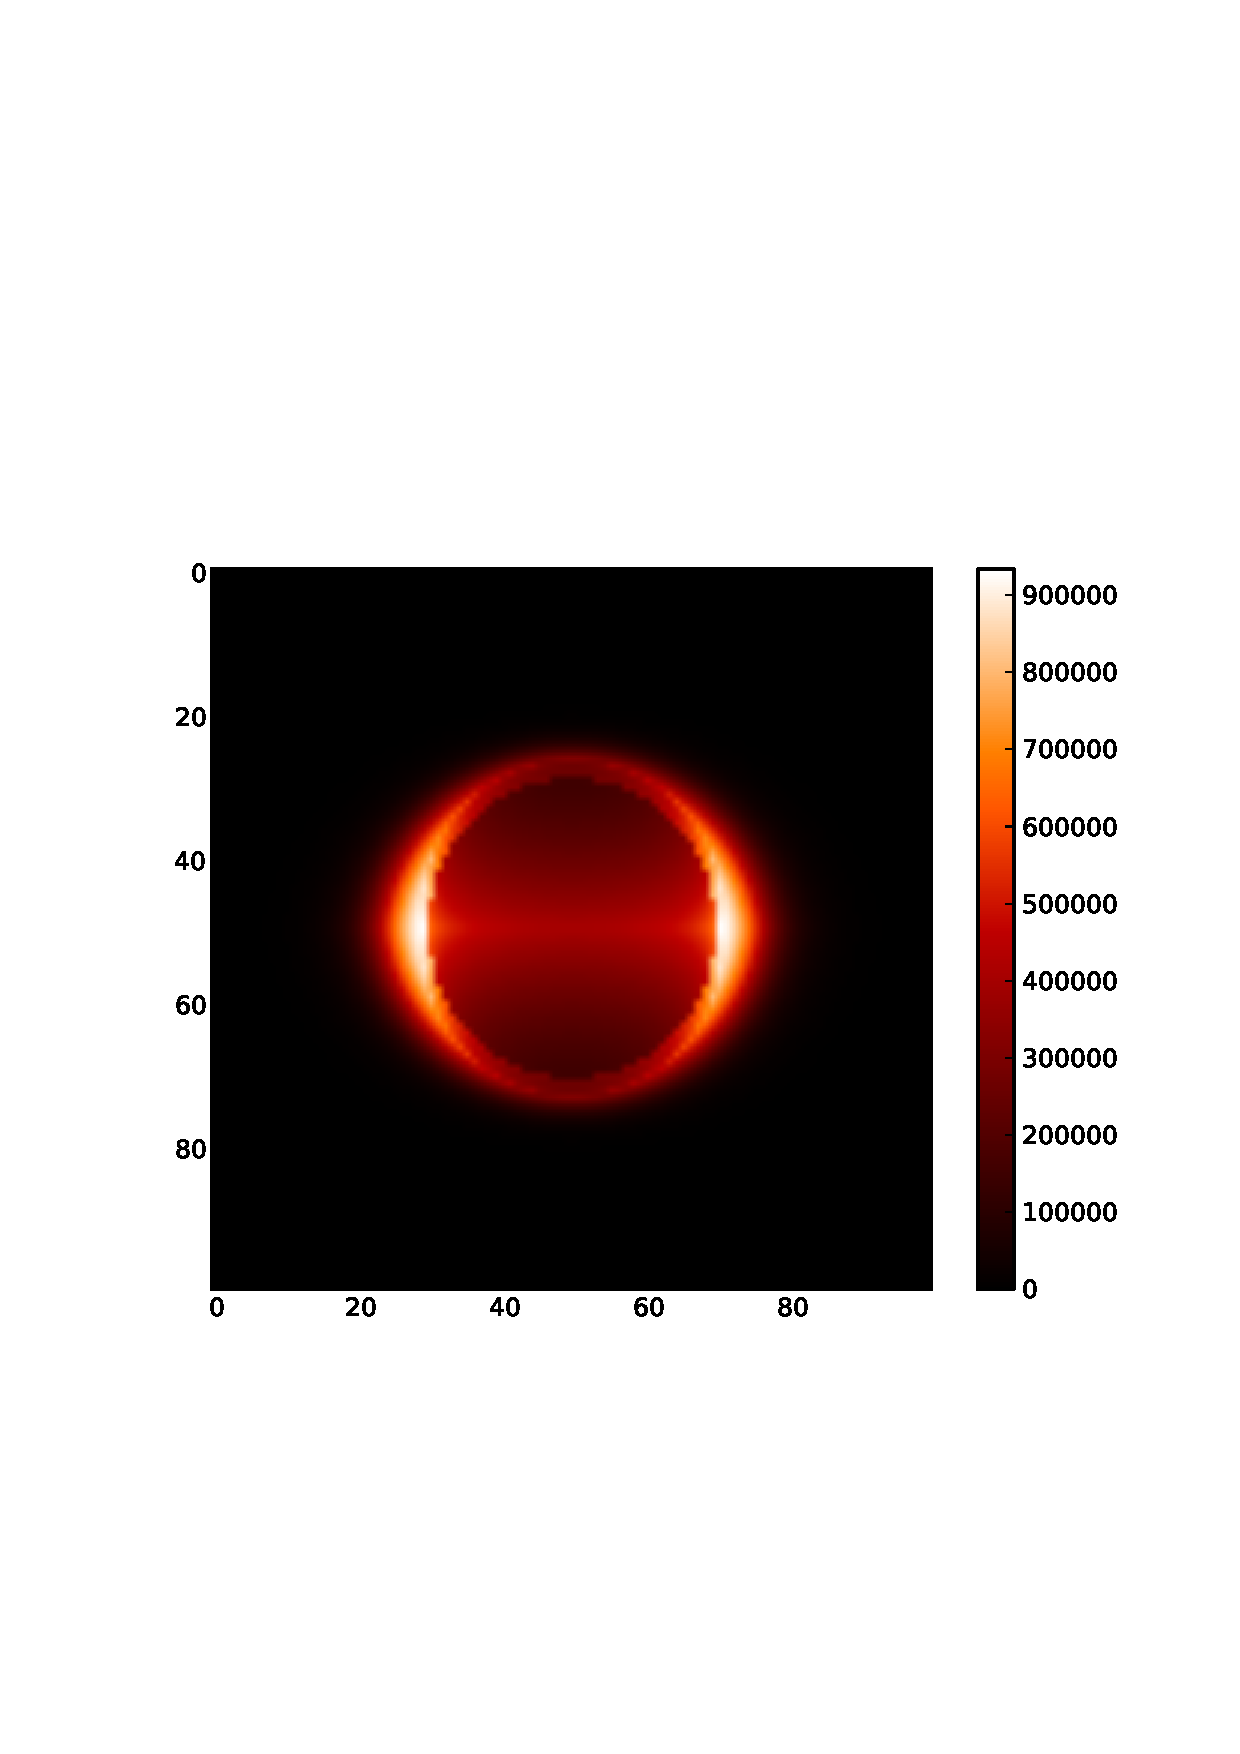
\includegraphics[scale=.75]{second_tbr}
\end{center}
\caption{This second image is of much better quality with a resolution
of 100, 100. It also changed the imageplane to include more of the sun
and less of the surrounding space. Furthermore by changing the
frequency we can see limb-brightening.}
\end{figure}

\subsection{Using all of ipython's tools}
The interactive Python shell provides the user many tools to interact with the
simulation. We will now consider some of these tools, however, only by
familiarizing oneself with ipython and pylab can the user take
advantage of all the tools ipython offers.

Lets begin with once again running a simulation.

\begin{lstlisting}
import raytrace as rt
implane = rt.implane(grid=(100,100),rect=(-2,-2,2,2),freq=300e6)
implane.trace(1500)
\end{lstlisting}
All the information for brightness temperature is now stored inside of 
iplane.tbr (or implane.tbriv if the mode was 'TbrIV'). This allows the 
user to directly access all of the elements in these arrays. Running
\begin{lstlisting}
implane.tbr
\end{lstlisting}
will display all of the elements of the implane.tbr array. To view an
individual element use implane.tbr[x,y] (or implane.tbriv[x,y,stokes]
where stokes=0 is I and stokes=1 is V).

If you want to view elements where some condition is held you can use
the numpy function {\bf where}.

\begin{lstlisting}
implane.tbr[where(implane.tbr>1000)]
\end{lstlisting}
Since {\bf where} returns the indicies of the array where the
condition is true. This displays all the elements where the brightness 
temperature is greater than 1000. 

Furthermore, using matplotlib the user can graph the data in many
forms. Visit \url{http://matplotlib.sourceforge.net/} to
learn more about graphing.


\subsection{Plasma Profile}
Beyond looking at the brightness temperature and stokes I \& V
parameters, it is also possible to examine the properties of the
plasma around the sun. This can be done by using the plprofile
function.

\begin{lstlisting}
import raytrace as rt
implane = rt.implane(grid=(100,100),rect=(-2,-2,2,2),freq=300e6)
p = zeros((100,3))
p[:,0] = linspace(1,5,100)
profile = implane.plprofile(p)
\end{lstlisting}
Lines 3 and 4 made an array of 3d coordinates where x goes from 1
solar radii to 5, with 100 steps. Now profile contains a tuple. profile[0] is
a one dimensional array of density, profile[1] is 3 dimensional array of
gradient of density, and profile[2] is a 3 dimensional array of the magnetic
field components. Now the user can explore these arrays to understand
how the plasma is structured around the sun.

\subsection{Streamers}
The ability to make streamers is an important part of the HART
package. The function rt.make\_streamer allows the user to add a 
new streamer to the sun. This streamer will then affect all instances
of implane objects.

The make\_streamer function has the following main parameters.
\begin{itemize}
\item Theta: Colatitude of the streamer (degrees)
\item Phi: Azimuth of the streamer (degrees)
\item Orientation: The orientation of the monopoles of the streamer in
  degrees where at orientation=0 the axis of the streamer is
  along lines of latitude, and at orientation=90 the axis of
  the streamer is along lines of longitude.
\item Density: The density of the streamer
\item BaseStrength: The magnetic field of the monopoles
\item StalkStrength: The magnetic field of the stalks
\end{itemize}

Applying this new function we can run a simulation with a streamer at
theta=90, phi=90.
\begin{lstlisting}
import raytrace as rt
implane = rt.implane(grid=(100,100),rect=(-2,-2,2,2),freq=300e6)
rt.make_streamer(theta=90,phi=90)
implane.trace(1500)
imshow(implane.tbr,cmap=cm.gist_heat)
colorbar()
\end{lstlisting}

\begin{figure}[ht]
\begin{center}
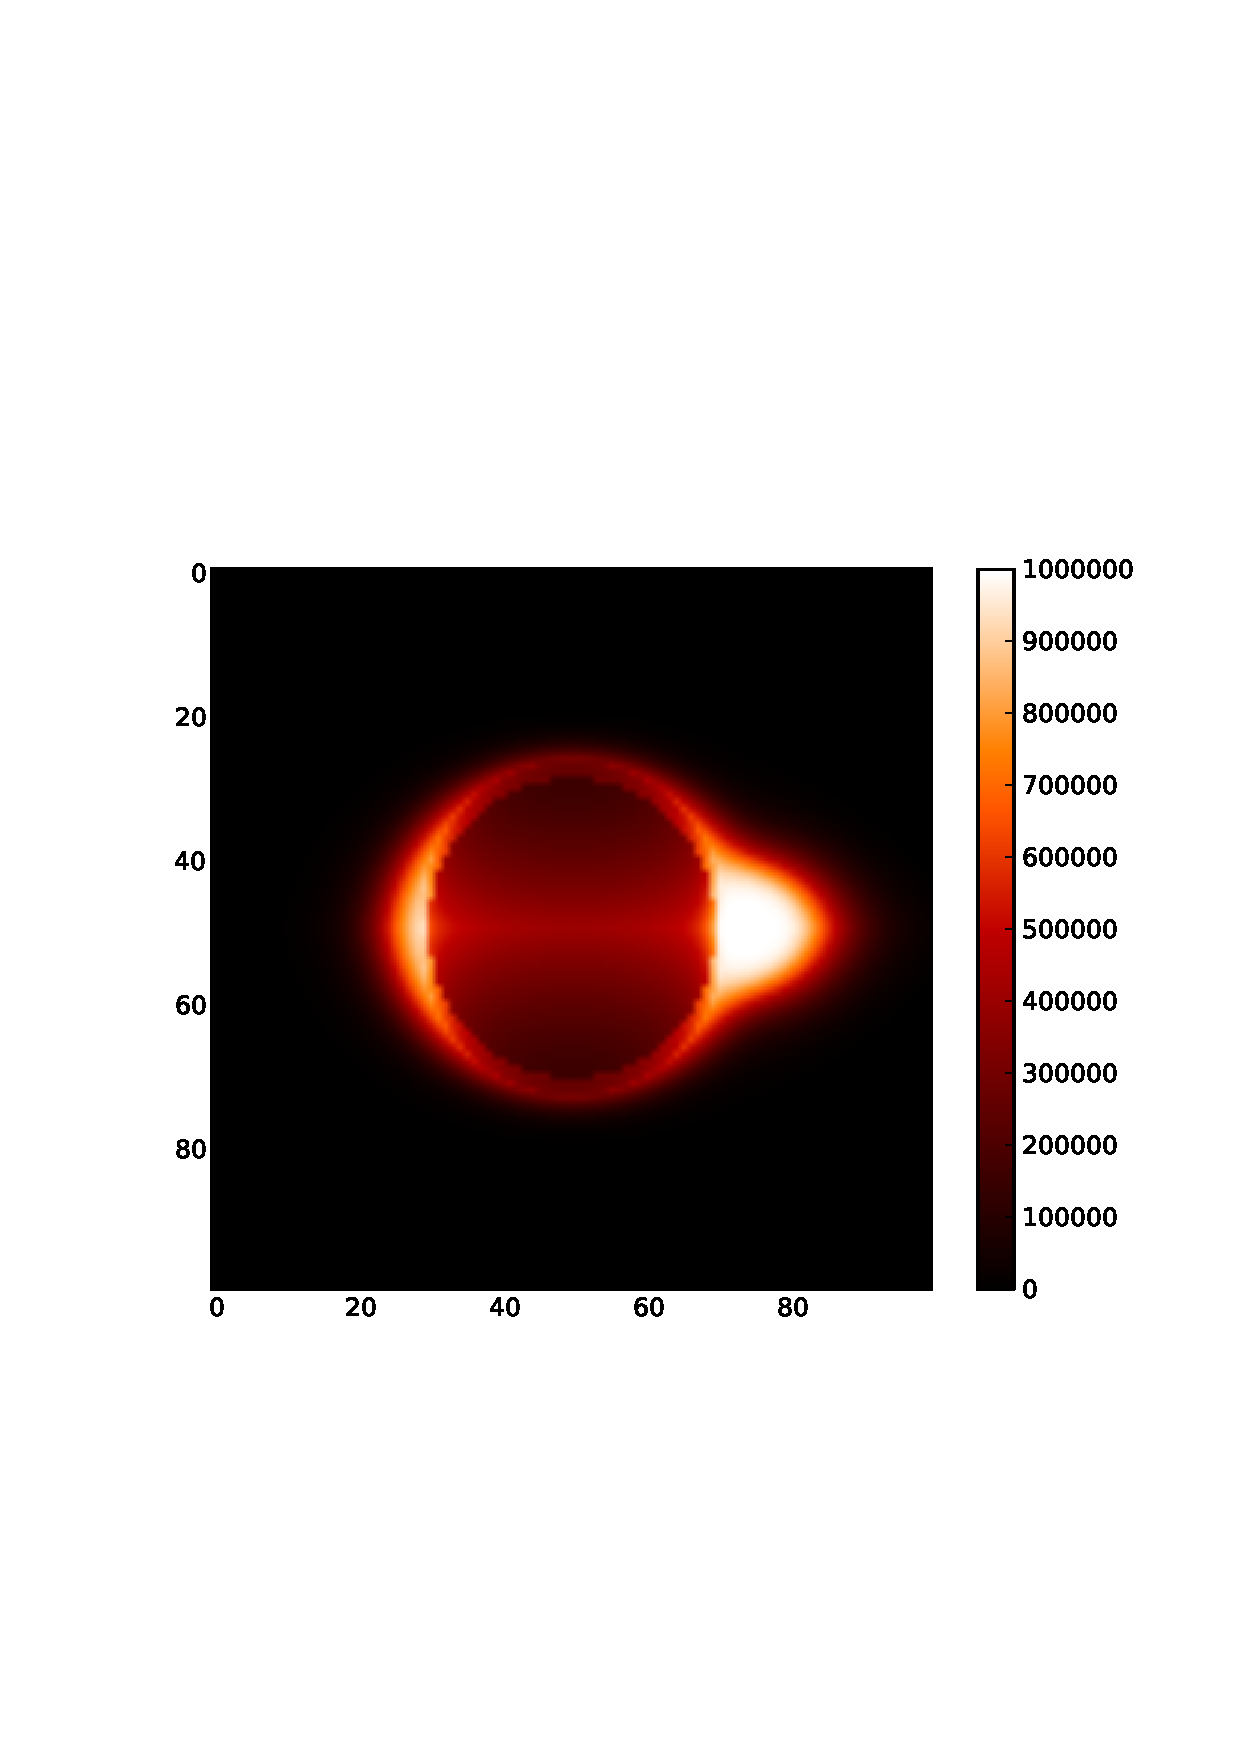
\includegraphics[scale=.75]{first_streamer}
\end{center}
\caption{This simulation shows a streamer at (theta=90,phi=90)}
\end{figure}

Running:
\begin{lstlisting}
rt.make_streamer?
\end{lstlisting}
will show the user how to use the more advanced parameters of
make\_streamer.

Now if the user wants to remove the streamers then he should run 
\begin{lstlisting}
rt.remove_streamers()
\end{lstlisting}

\subsection{Advanced Features}
Advanced features will be discussed in {\bf \autoref{sec:6}}. Now however,
we will examine the use of the GUI to interface with the simulation.

\section{Using the GUI}
Because simulations often require many repetative tasks, we have
implemented a GUI in order to reduce the time needed to perform the
more mundane tasks. However, using the GUI removes the user from
the data, making it more difficult to inspect individual elements. 
Later, we will consider running the GUI through ipython in
order to get the advantages of both. But first, let us examine the GUI
and how to use it.

\subsection{First Trace}
Launch the GUI by running gui.py. Once launched change the selection
from basic to tbr and then click ``Trace''. This will perform the
simulation. Once completed you can press ``Tbr Graph'' which will
display the brightness temperature.

Changing the parameters on the gui will affect the simulation as
described in section {\bf \autoref{params}}.

\subsection{Trajectories of Rays}
It can be useful to see the trajectories of the rays you are
tracing. Although this is possible through ipython, it is
significantly easier to perform through the GUI.

\begin{figure}[ht]
\begin{center}
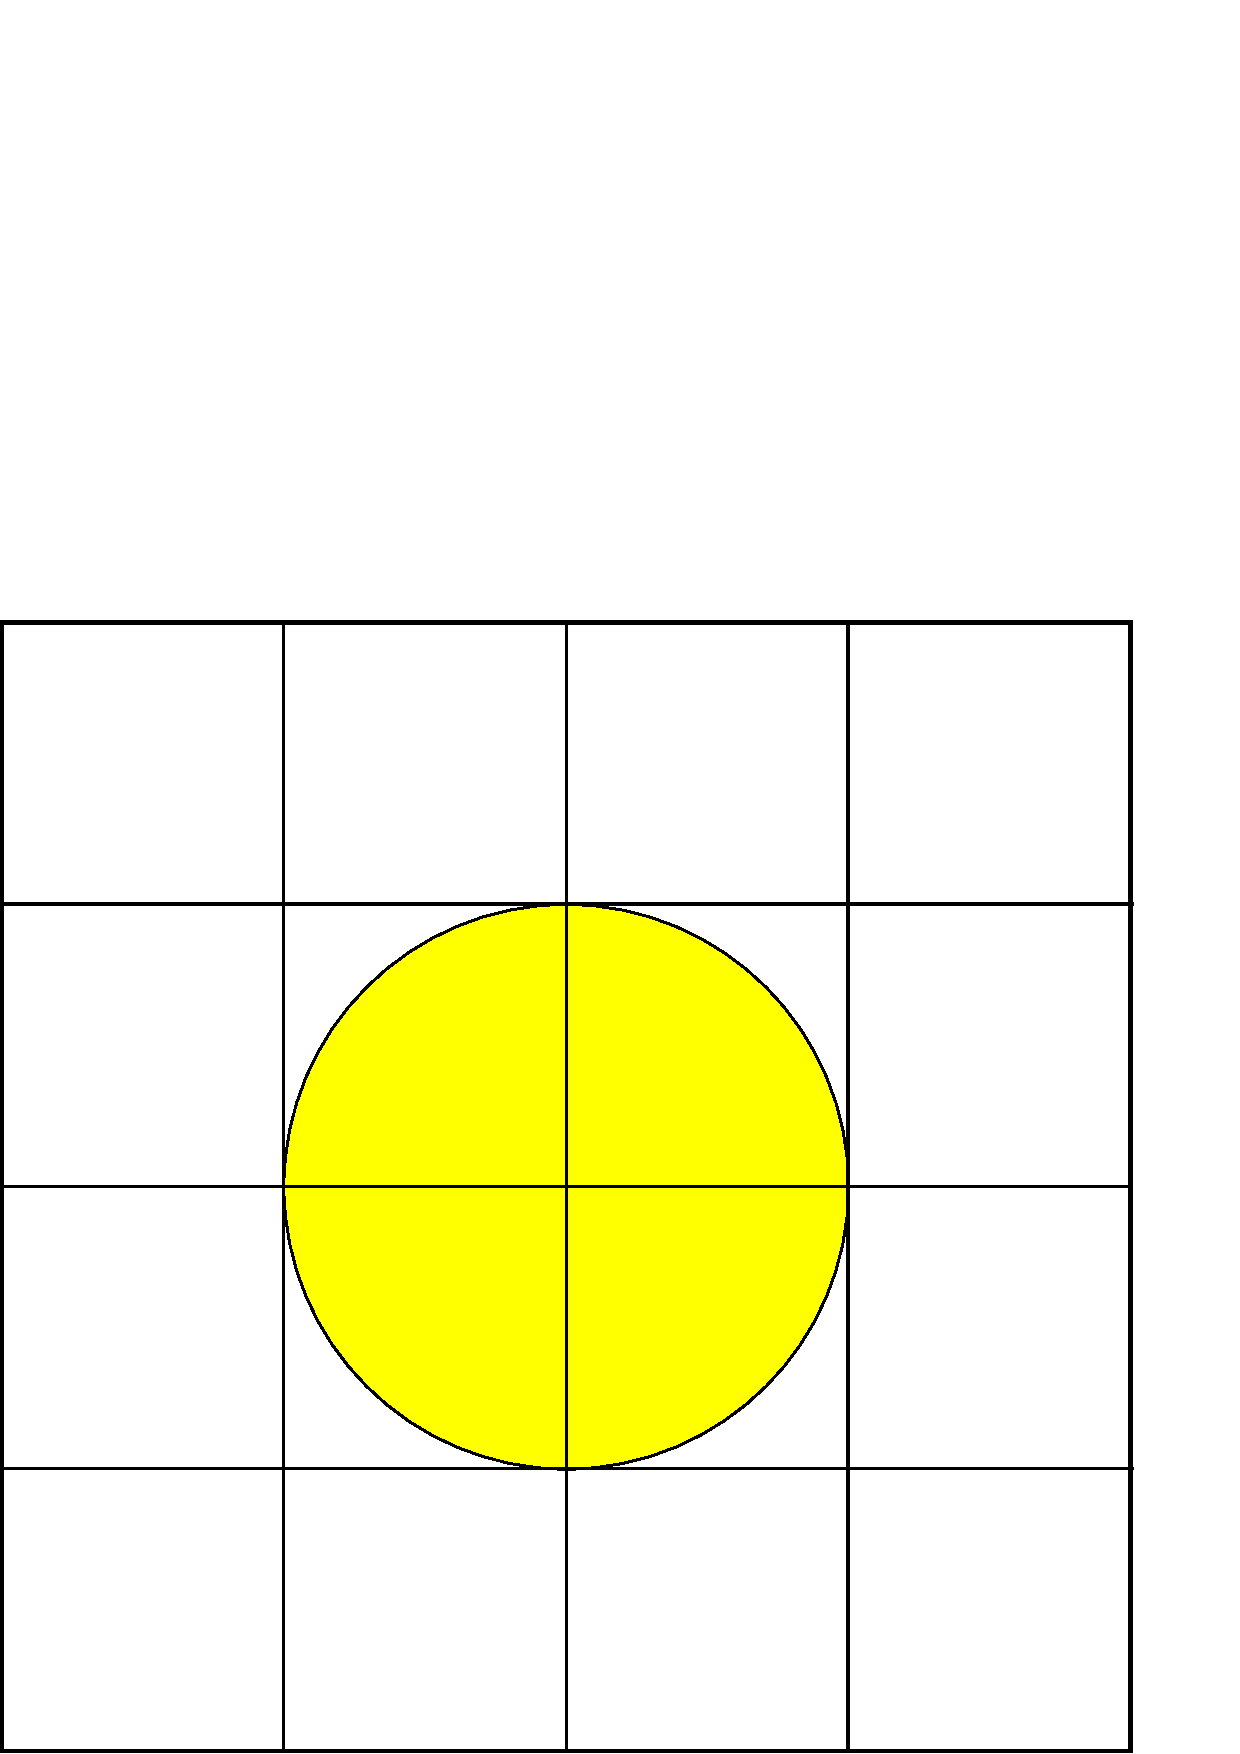
\includegraphics[scale=.5]{trajectory}
\end{center}
\caption{The grid from the GUI.}
\end{figure}

Every grid square represents one of the rays to be traced. Clicking on
a grid square means that ray's position will be stored at every point
to provide the user with the ray's overall trajectory. If any of the
grid squares have been selected then once the trace has been
completed, pressing the ``Show Trajectories'' button will show the
trajectories of all of the rays.

At the bottom of the solar grid, there are two buttons that can help
select which rays to trace. ``Clear'' removes all selections, while
``Select All'' selects all of the rays for tracing. Furthermore, right
clicking on a square will deselect that ray, meaning that its
trajectory will not be recorded.

\subsection{Adding Streamers}
Adding a streamer is very easy. Click the ``Add streamers'' button in
the middle bottom of the window. Then place the streamer by clicking
on the image of the sun. You can change the streamer's orientation by
using the mousewheel. When you click to place the streamer, the
program will ask you if you want to change any of the
parameters. After that you can place more streamers. When finished,
there are two possibilities. Hitting ``cancel'' will remove all of 
the streamers, and ``ok'' will place the streamers. After running 
a simulation, all of the streamers will automatically be removed.

\subsection{Step Mode}
Finally the GUI introduces a step mode feature. In this mode, it is
possible to see the rays go through every step of their trace. To
begin this mode, click on the ``Step Mode'' button on the left. You 
can now click forward to advance the specified steps. At each
juncture, the current graphs of brightness temperature or stokes 
I \& V will be shown as well as the current position of all of the rays.

You can also examine a ray (which is highlighted in red). By giving
the grid coordinates of one of the rays. The density, gradient of
density, and bfield will be displayed for the given ray at the given step. 

\section{Making a FITS File}
One advantage of HART is the ease with which FITS files can be
made. This is most easily done from some outside python file that
calls the raytrace module. Consider the following program.

\begin{lstlisting}
import raytrace as rt
import numpy as np
import math

rt.run_freq_range(file='data/scattering',grid=(300,300), mode='Tbr',
                  steps=12,scattering=True)

th = 60
pi = 90
rt.run_freq_range(file='data/theta'+str(th)+'_phi'+str(pi),
                  theta=th,phi=pi,orientation = 0,grid=(300,300), 
                  mode='Tbr',steps=12,scattering=True)
\end{lstlisting}
The run\_freq\_range function runs a simulation for many frequencies
and saves the result in a FITS file specified by the parameter {\bf
  file}. The first call to the function will save the fits file in the
directory ``data''. It will be on a 300x300 grid with 12 frequency
steps between the default 80MHz and 300MHz (i.e. every
20MHz). Finally, scattering will be turned on. The second call to the
function does a very similar run, except that there is a streamer
placed at (90,60).


\section{Advanced Features}
\label{sec:6}
There are a couple of more difficult features that were omitted when
initially talking about the ipython shell. We will now discuss these
and examine how to use them.

\subsection{Trajectories}
Just as it is possible to see trajectories through the GUI it is
possible to also see trajectories through ipython. In order to do
this, an array must first be created which contains the locations of
the arrays that should be kept track of.

\begin{lstlisting}
import raytrace as rt
implane = rt.implane()
p = empty((n,2))
\end{lstlisting}
where n is the number of rays to track. Then every ray you want to
track should be indexed with an x and y coordinate in the p array. For
example if n is 2 then the following will trace the rays starting at
(2,2) and (8,8).

\begin{lstlisting}
p[0,0] = 2
p[0,1] = 2
p[1,0] = 8
p[1,1] = 8
trajectories = implane.trace(1500,p)
\end{lstlisting}
Where trajectories stores the calculated trajectories of each of the
rays specified by p. If a ray finishes early, it will contain NaN's in
the rest of its trajectory to indicate that those values would
otherwise be meaningless. These trajectories may now be graphed use matplotlib
or examined through ipython.

\subsection{The Value in Trace}
We have called trace numerous times. We always include a value, but
never explained what it actually is. That value is the upper limit on
the number of steps the simulation can take. The default value is
100. Usually without scattering 1500 is a safe number to choose. With
scattering it can take closer to (at least) 3,000, or may never completely
finish. After completing a trace, the program reports how many rays
are remaining. If desired the trace function can be run again in order
to complete the remaining rays. Or if enough rays have finished the
data can be accessed. One disadvantage of the GUI is that currently it
completes a maximum of 3000 iterations and there is no way to perform
more.

\subsection{Running the GUI Through Ipython}
First run ipython, then type \%run gui.py. This launches the GUI from
the shell. Now the user can use the GUI normally but also access all
of the data inside. The implane object the GUI uses is accessible from
main.trace so that main.trace.tbr will store the data and
main.trace.trace(1500) will perform a trace. This combines the ease of
the GUI with the powers of ipython.

\section{Speed Improvements}
One of the advantages of HART is the fast algorithm as well as
multithreading and CUDA. Through these two technologies, HART can make
use of both many proccessors and graphics cards.

\section{Plasma Parameters}
It is possible to change the models that define the solar
plasma. Currently the plasma parameters file uses the Saito Model for
the density in the Solar Corona, and a stitching function to combine
that with a chromospheric model. As better models arise, these can be
easily inserted into plasma parameters. Then using the
set\_plfunc(filename) function in ipython the simulation can make use
of the new plasma parameters file. This file can also be compiled from 
the GUI by clicking on the recompile.


\end{document}
